\documentclass[11pt]{book}
    \title{\textbf{Ana} \\ \vskip 1em \small The policy of silencing}
    \author{Tatiana Balbi Fraga}
    \date{}
    
    \addtolength{\topmargin}{-3cm}
    \addtolength{\textheight}{3cm}
    

 \usepackage[T1]{fontenc}
 \usepackage[utf8]{inputenc}
% \usepackage{amsmath,amssymb}
 %\usepackage[T2A]{fontenc}
 %\usepackage[russian,english]{babel}
 \usepackage{graphicx}
 
\begin{document}

\maketitle

\chapter*{Abstract}

'Ana: The Policy of Silencing' is a book that discusses some important issues of our century, such as: COVID; technological advancements; the loss of privacy and individuality; immediacy; competition; the industry of madness; posthumanism; transhumanism, etc. \\

\noindent The book uses an adaptation of the textual language used by Laura Nowlin's in her book 'If He Was With Me'. Nowlin narrates the past using present and future time. It's interesting. \\

\noindent However, the idea of the book is to design a web of memories and reflection, creating a story that walks through a brain's synaptic networks... \\

\noindent It is not possible to know if it will be good until it is over. \\

\noindent And there is no intention to finish it. \\

\noindent In short ... it's just something for distraction ... but also a provocation in the hope that things will change at some point. \\

\thispagestyle{empty}

\chapter{about being alone}

I have always loved silence and tranquility. So being alone has never been a problem for me. Even isolated, I never felt really alone. \\

\noindent I once saw a report on TV5. The interviewee was a lady who was about 50 years old, with very short dark hair. This lady said she liked to go to a isolated place and be alone from time to time and that her family was unable to understand it. Trying to explain the feeling she sought, she said:

\noindent \begin{center} "Only when I'm alone I can find God." \end{center}

\noindent I could completely understand this lady. I thought: That's right. But, it was in recent years that I understood what it means to be alone...

\noindent \begin{center} \emph{Being alone means living the horror and having no one to ask for help.} \end{center}

\chapter{Sweetie}

\noindent It happened more than once. But the first time was something different. I was driving with a kitten on my lap. And submly I started to see the world with a different color. It is a subtle joy, without any foundation. A supreme well -being, a contently for nothing and anything. \\

\noindent The kitten was all black, very small. It was still a baby. In the corridors of universality. Someone passed and it followed the person. Then it came back to the same point, just to follow the next passer again. \\

\noindent There were many turns, until someone felt a strong interest in the kitten, and stopped to observe it with a certain curiosity. \\

\noindent I asked: Do you want to adopt it ? I promise that I give it to you castrated and dewormed. \\

\noindent Then I saw on her face a wide smile of comtemplation. \\

\noindent The kitten is so sweet that I named it Sweetie. I left Sweetie in my room at work until the end of the day. I tried to use a cardboard box to transport it to my house. But it ran away and while I was driving, Sweetie came to lodge in my lap. \\

\noindent I remember how happy I was, driving toward my house with that kitten. \\

\noindent In the following days, I cast it, and we spent a long time together until its complete recovery. Sweetie was very \emph {sapeca}. She was terribly happy at home. \\

\noindent The days passed and I had to take Sweetie to its new owner. It was a little sad. Leaving Sweetie was very painful. It was like leaving a part of me. I donated the transportation box along with the kitten, and half a feed bag so that Sweetie could adapt well to its new home. \\

\noindent I said to my husband, Adan: I hope God takes good care of Sweetie. He replied: He is already taking care of. \\

\noindent Later, Sweetie recovered its old behavior. Someone passed and Sweetie followed the person, and returned again to the grocery store, just to follow the next person. Sweetie had to deal with another somewhat territorialist kitten. Its new mate did not want to share the love of its owners. \\

\noindent But Sweetie had its destination adjusted. And was adopted again. In Its new home, Sweetie found the company of a child. And happiness found both. Today Sweetie is a very loved and happy kitten. It's already adult, but it's still \emph{sapeca}. When its owner arrives home from college, Sweetie lies next to her. And keep looking at its owner typing on the computer. At night, Sweetie lodges on the feet of the bed. Look at its owner sleeping, gives a long supply and closes its eyes, waiting for the next day to arrive. \\

\chapter{The Covid Gang}

\noindent In spring, the heat came back in all its fullness. I decided I should put my concerns aside and go for a walk on the beach. After all, I left my apartment abandoned for a long time. I thought I deserved to take care of myself and that after a day or two on the beach I would be much more willing. \\

\noindent Friday was a perfect day. The trip to the beach was very fast and calm. Many people in the sand and many boats in the sea. All very different from what I remembered. But the day was beautiful. I walked all day in the beach sand and took a sea bath surrounded by fishes. I ate fish with capers sauce that was delicious, in an expensive restaurant . I bought a pot of acai that served to dinner. I read a little more of Laura Nowlin's book "If he was with me" while lying on the net. Everything was great. At night I slept like a stone. \\

\noindent On Saturday things change completely. Mr. Marcos da Fonte was an acquaintance. I found him casually early in the morning, while arguing with the doorman about the real need to have some kind of registration. I talked to Mr. da Fonte about condominium issues and told him about my kidnapping. \\

\noindent In the afternoon I'm reading on the net, and then suddenly I start to feel a terrible discomfort. I feel a very strong pain in the nostrils and a severe headache. Through the crack of the door, I see the cleaning lady passing cloth on the floor. \\

\noindent The malaise only increases and I decide to return home. I was thinking of leaving only after noon, but I advance my plans. Arriving at the post, I take a bottle of Gatorade at Freeser and ask for a cheese bread. I'm really feeling nauseous, as if I had drunk alcohol all night. It's been a long time since I've been drinking anything alcoholic, but the feeling is familiar to me. The boy takes my cheese bread through the door to warm it inside the kitchen. I think it's weird. I ask him why he didn't use the oven or the microwave in the canteen itself. He makes some not very reasonable excuse. \\

 In the middle of the trip, I enter a local avenue. I remember there was a supermarket I visited two weeks ago. As soon as I enter the avenue, a SAMU's vain comes out of somewhere and goes in front of me. I repeat to myself: just ignor it. And I follow my way ... \\
 
In the supermarket, as usual, there was an employee changing some cans, near the place where the mineral water bottles are. I see some crates of the bottle that I usually buy on the floor, next to this boy. On the shelf there were a few bottles like these. The bottles were covered with dust, as if they were there without care for a long time. Then I chose a different brand. I took some bottles that were not dusty. Almost arriving home, I stop in a good restaurant. I feed well and malaise passes the same time. While how, I see the attendant leave the counter a little stunned to talk to someone who seems to be the manager. I hear part of the conversation. The attendant says: she doesn't ... The alleged manager makes gestures and tells the attendant that he should move the food.\\

\noindent I get home and I feel relieved. Nothing better than being at home. I take a shower and take the book I was reading. After all, I really wanted to finish reading the book. I lie on the porch couch and start reading. \\

\noindent After a few minutes of reading, some car at a reduced speed is on the road with the sound really very high. I stop reading a little and listen to the lyrics of the song that plays: "Take it, take it, take it in the ass." I have the impression that the car has stopped, because I hear the sound at the same height, without the sensation of which it is moving away. The chorus repeats himself a few times: "Take it, take it, take it in the ass." I try to ignore and go back to reading and then I realize that the volume of the sound slowly reduces until disappear. \\

\noindent The night is not very pleasant. I wake up feeling pain and discomfort again. It's still dawn. I hear some sound and decide to walk inside the condominium to find out where it comes from. I walk the condominium road following the music and find that the very high sound is installed in a narrow little deforested dirt road next to the condominium fence. I come home, I repeat to myself that my house is the safest place in the world and then I sleep again until morning. \\

\noindent On Sunday, I take the day to write and hear a cyrene sound on the road several times throughout the day. It bothers me a little, but I try to ignore it.

\chapter{Adam}

\noindent We are walking in the beach sand in Mikonos. We see a great rock a little distant from the coast, as if it were a small rocky island being snatched by the sea. Adam propose that we swim to the island, and of course ... I would never refuse. \\

\noindent Sea water is warm and transparent. We are wearing diving glasses and we swim to the island, submerged and hand in hand ... \\

\noindent The island is a little larger than I expected. We explore the island and, like two children, we try to hide when we see a boat coming close to us. \\

\noindent On the way back, I dive into the sea with my hands forward, as if I were a dolphin. But I do this wearing the diving glasses that break when shocking with the water. I swim to the coast with my forehead bleeding, but with a big smile on my face ... \\

\noindent Weeks later, we are already back in France ... I walk next to Adam ... \\

\noindent Adam tells me about a recent dream. He tells me that we are walking hand in hand on the sea, as if we were walking on a thin, transparent layer of ice. And that, under our feet, we can see thousands of fish. I can see Adam's dream like a memory. \\

\noindent I have no doubt about the meaning of the dream. It is just a reflection of the feeling we have for each other.

\chapter{Day before my kidnapping}

\noindent After driving many hours, I arrive at my beach apartment accompanied by my mother and my cousin, Basco. I am really exhausted and I feel that I will have difficulty giving the medication to my kittens. I let out the kittens in the bedroom and, with a lot of effort, I put the sandbox, feed and water for them and I can medicate Braquinha and Lucy. Then I fall on the bed and finally sleep like a stone. \\

\noindent I wake up after several hours, feeling very hot. I'm still really tired. The deep sleep I had was not enough to recover my disposition. The room is muffled, in a way that cannot be supported. I open the bedroom door and I free my kittens in the apartment.  \\

\noindent I walk to the living room and see my mother lying on the bicama couch. She has a somewhat strange expression, as if she was feeling terribly terrible with something. Basco is not in the apartment. The kitchen sink drain is covered with a water-filled cuzcuzeira, and the bathroom sink drain is clogged with colored toothpaste. The sink is full of water. Given what I've been through in recent days, I didn't find it strange. But I said to my mother: Mom, the kittens are drinking water from the bathroom sink ... this will make them sick.  \\

\noindent My mother goes to the bathroom, empties and cleans the sink. \\

\noindent Hours later, several people arrive at the apartment door. My mother opens the door and a slightly strong gentleman with a somewhat rounded face crosses the door. My mother leaves the door open as Mr. Rounded Face begins to question me, without worried about a possible glow of my kittens. A condominium employee awaits outside, accompanied by unknown persons. I am worried about the door open and my kittens, but the lord with rounded face begins to question me abruptly. \\

\noindent I tell this gentleman about why I want my mother to leave. I answer the questions narrating a long story. Although I am confused with what was happening, I came to some kind of conclusion. \\

\noindent When he finishes his interrogation, Mr. Rounded Face turns to my mother and says: we can't take her like this, she's fine. \\

\noindent The people who were outside move away. Mr. Rounded Face begins a somewhat strange speech. He proposes that I walk on the beach with my mother so someone he has entitled "she" couldn't hear us. My mother has an espression that becomes more restless as the Lord's speech continues. Then he closes the door of the apartment and says: Since your mother is here, I will say: Don't exceed yourself because we will make you suspect everyone.  \\

\noindent I don't know what to think about all this. Nothing seems to have some kind of coherence, but I try to put the facts together. \\

\noindent My mother is washing dishes and I stop by her side and ask: is you the person responsible for all this ? \\

\noindent My mother bends her body down forming on her back a hunchback. She tilts her head to the side and down. Then she shakes her head positively, speaking softly: Yes, it's me. \\

\noindent I tell my mother: I want you to leave. \\

\noindent And my mother resists with a certain insistence. \\

\noindent After a while, my mother gives me the phone, saying that I should talk to my sister. \\

\noindent I say on the phone: Thaila, I want mom to leave. And Thaila replies: Ana, you have a niece. Confused, I return the phone to my mother and say: You leave. \\

\noindent After a few minutes my mother comes to talk to me. She says: I'm leaving tomorrow, but only if you talk to a doctor. He will call at 19:00h. \\

\noindent We await the call, the doctor does not call at 19:00h and he does not call later. I tell my mother: Well, no doctor called. And my mother replies: he may have suffered an accident. Again confused, I say: I already waited enough, I'm tired, I'm going to sleep. Tomorrow you leave. \\

\chapter{Genius and madness}

\noindent Many people believe that genius is a gift that arises when geniuses are born. But this is not totally true since every being is the result not only of genetics, but also of a set of experiences. \\

\noindent I believe that:

\noindent \begin{center} \emph{Genius happens after total abdication of itself through self-delivery to a passion for which the genius being has aptitude} \end{center} 

\noindent In history, many geniuses are portrayed as crazy at some point in their lives, as exemple:

\begin{itemize}
\item During his doctorate, and before redefining Game Theory, John Nash talked to invisible people; 
\item In the last years of his career, Albert Einstein used to go to work using pajamas. 
\end{itemize}

\noindent I will not comment here that, in 1994, John Nash was awarded the Nobel Memorial Prize in the Economic Sciences for his contribution to game theory. \\

\noindent About Einstein, I feel as if I knew him deeply and I can guarantee that going to work wearing pajamas was for Einstein a form of mockery to society's standards. \\

\noindent For a long time, Einstein's brilliance was deliberately hidden due to the envy of co-workers. After many years he was finally recognized and became a key element for the university's image he worked for. Einstein had numerous scientific publications and discoveries that changed a generation. Therefore, when Einstein understood that his place in the world was already sealed, he became a better version of himself, abandoning behaviors that were now dispensable for him. \\

\noindent The story of these crazy geniuses brings out an important question: what is madness ? \\

\noindent And, based on my recent experiences, I can present a possible answer:

\noindent \begin{center} \emph{Madness is a behavior that is not accepted by an elite of the social group in which the madman is inserted.} \end{center}

\noindent From the madman begins to emerge new ideas and questions related to standards, ethical questions, principles and truths. Concepts which such an elite does not want to dig up.

\noindent \begin{center} \emph{Madness is therefore a way to silence the provocations of a genius} \end{center}

After all, attesting that a person is mad, it is a very effective way to discredit them.  \\

\noindent One thing is certain about the geniuses:

\noindent \begin{center} \emph{A genius sees things that other people can't see, in places where other people don't expect} \end{center}

\noindent So it is natural for genius people not to be understood. And the fact that geniuses are always linked to change, it can really scare. \\

\noindent Therefore, people's cruelty is not associated with fear or lack of understanding.

\noindent \begin{center} \emph{People's cruelty is linked to the cruel, selfish and competitive nature, inherent in the human being.} \end{center}

\noindent And madness is clearly a concept created by cruel people.

\chapter {COVID Gang - Who are they ?}

\noindent When you think of COVID, you cannot see this in a purely personal aspect ... But in fact, COVID has become personal for thousands, millions or even billions of people. COVID didn't just happen to me. But it happened to me lately in a way as inhuman and frightening as torture and terrorism can be. \\

\noindent Thinking about the personal aspect, the COVID Gang can be distributed in two classes: people who are financing the aggressions; and people who are performing the aggressions. \\

\noindent Who are the people who are financing this ? \\

\noindent I paid an appointment to two lawyers. I told them about the last torments I have had to endure. \\

\noindent We are in our third meeting and the lawyers have a budget in their hands. The lawyer tells me: I believe that who is doing this is a group of people. \\

\noindent The lawyer is right, but who are these people ? \\

\noindent In my opinion, if it is really a group, this group could be formed by: owners of a psychiatric clinic, employees of a technology company, people from my work; other public officials; a corrupt lawyer I hired in the past; people from my beach condominium; the construction company that sold me the beach apartment; person who sold me the land in which I built my house. Most of these people, assaulted me strongly in very different ways, long before COVID begins. These are the people who might want to silence me or make me look crazy and disappear, buried alive in a clinic.\\

\noindent And who are the people who are directly terrifying me ? \\

\noindent Criminals and ordinary people who are unemployed or earn a low salary such as cashier attendants, truckers, restaurant employees, gas stations attendants. \\

\noindent It is possible to understand why the "hate financiers" are assaulting me. \\

\noindent But why do ordinary people are assaulting me ? \\

\noindent There are many possible reasons, but I have some guesses that seem to present some kind of logic:

\begin {itemize}
\item some people have been hired in some way for this;
\item someone created some kind of hatred chain against me;
\item criminals are assaulting other people and making it seens that I am responsible for this;
\item criminals are assaulting or threatening other people who refuse to assault me;
\item Some people just feel good about doing this.
\end{itemize}

\noindent Possibly all these alternatives are correct. The only thing I can think is that somehow people were convinced to cooperate in this regard. \\

\noindent This is the logical conclusion that I arrived after almost two years being tortured and terrified. But ... is there any other explanation behind it ?

\chapter{A good opportunity}

\noindent It's been over a year since I started my doctorate. Nancy is an excellent workmate. It's been a few years since we started working in the same room. We divide our dawn in front of our computers ... reading ... typing ... searching. We have different goals for a common end: research. And it seems clear, we love what we do. \\

\noindent We talk little, but our short conversations are always pleasant. We talk about our lives, the longing for a daughter, the need to pay bills from a distant country ... We live in a small town, but we never talk bad about other people. \\

\noindent Nancy always gives me some important tips that I will lead to the rest of my life, such as about CodeBlocks, cplusplus.com, or about some technical concept or even how to overcome some buracratic challenges of the university. \\

\noindent We are on a cold night squeezing our arms under our already aged wool coats. Nancy tells me about doctoral scholarships abroad that are offered by Capes and CNPq ... \\

\noindent I always wanted to know Europe. Especially Greece. I saw a few Greek movies, and I was always dazzled by the scenes that happened in the Greek rocks. Always an amazing landscape. And ... well ... the gods are Greek. \\

\noindent For this reason, I spent the next few days trying to understand a vast paperwork of edicts. \\

\noindent Then, I visit my advisor's room with a simple task: teacher, there is a doctoral internship bag abroad, I need you to present me a reference from someone you have worked with. \\

\noindent And he answered me: there is a teacher in the USA, another in Portugal, and finally, Professor Bernardo, who works at a university in France. \\

\noindent USA... no, no, and no ... Portugal ... all there they speak Portuguese ... \\

\noindent The next days were nothing easy ... \\

\noindent I'm crying in front of the computer because I don't understand the meaning of \emph{on}, \emph{y}: \emph{On y vas ? On a parlé.}  \\

\noindent I have little time. I need to take a grade 7.0 in the French Alliance test. Toffel-equivalent examination for the french language. \\

\noindent I paid a few classes to a French teacher. She gave me some important tips on TV5 and a French radio. But after three meetings, she told me very sincerely: you won't make it. \\

\noindent At this point I introduce something very important about my personality: In my life, I never measure efforts. \\

\noindent I create a learning technique totally outside any standard of reality. \\

\noindent I chose some videos from the channel apprende TV, from the TV5 website, so I decide to listen to the videos, then read and translate the transcription, then listen again, then listen and write. I make it repeatedly, until I could understand speech and write the  text 100\% in french without any grammatical error. Then I start doing the same with french radio audios nominated by the teacher. \\

\noindent After three months repeating this repertoire, I perform the French Alliance test. And my grade is: 6.5. \\

\noindent I'm a little unhappy, because I just have one more chance.  \\

\noindent I make another appointment with the French teacher. After all, the tips she gave me helped me a lot. \\

\noindent After a few minutes of conversation in french, the teacher says: I'm surprised. How did you get this ? \\

\noindent I answer: following your tips, and making an absurd effort. \\

\noindent After another month, I perform the French Alliance test again. And my grade is: 7.5. \\

\noindent And at this point I introduce other very important thing about me: I could never ever correctly pronounce the word \emph{apprendre}. Can anyone do this ?

\chapter{COVID}

\noindent I'm working in my bedroom. Adam calls me with a certain enthusiasm. I go to the TV room. Adam shows me a video of something that happens in China. People are leaving some city. The temperature of each person who goes through some kind of portal is measured with some instrument that seems to have the shape of a bar code reader. \\

\noindent I try to understand the English report with a certain effort. I understand part of the speech. The scene I see seems to repeat some movie about the Holocaust. \\

\noindent Adam tells me: How is it possible that they are letting people get out of town ? \\

\noindent I go back to my room and I Google the word sars cov virus. \\

\noindent I read some reports about Asian influenza and I try to understand as deeply as possible the type of viruses being addressed in the report. \\

\noindent I go back to the TV room, and I keep looking at the report next to Adam, now completely stagnant.

\chapter{Mr. Rocher}

\noindent I wake up at dawn feeling a severe headache. I swallow a pain medicine along with some sips of water. I turn on my computer and log into the game to do some missions hoping the pain pass. I'm really sleepy. I want to go back to sleep, but the pain bothers me. \\

\noindent Mr. Rocher soon finds me online and asks: Are you awake ? I answer: I have a headache, I can't sleep. \\

\noindent We talk about something of the game. There will soon be a battle between servers. Mr. Rocher is one of the first covenant ministers. He is responsible for diplomatic matters and is always solving disputes and seeking agreements. However, as one of the first ministers, he is also always concerned with battles. \\

\noindent I just adore him. While we talk I feel calm, safe and happy. \\

\noindent It's been about two years since we met. Our wedding happened a few months after someone decided to turn the game into a relationship site. Several wedding packages were launched with real prices varying according to the size of the party. We got the cheaper package, but we had a typical Russian wedding, with a lot of greetings and long verses with good fortune and a lasting relationship desires. It was a very funny, cheerful and even a little exciting moment. It was my first marriage. \\

\noindent After long minutes of a very pleasant conversation, we say goodbye long and then, without any trace of headache and with a wide smile on my face, I can go back to sleep.

\chapter{Kidnapping day}

\noindent I wake up in the morning. Basco is lying on the net. But soon he goes out to walk on the beach and I lie down where he was. \\

\noindent I sleep a little and wake up with my kitten Sol licking my hand. Very sleepy I see that the glass window that separates the room from the porch is slightly open. Still sleepy, I return Sol into the apartment and I close the glass window. I go back to sleep and again I wake up with another kitten licking my hand. Now it's Charlotte. \\

\noindent Now I realize a danger that represents finding my kittens on the porch and I wake up and raise scared. I tell my mother: Why are you releasing the kittens ? \\

\noindent I hear Mel meowing and see it on the bathroom box, as if it is very scared. My mother says: It's not me. They are leaving from the bathroom window. I reflect a little. The glass door was a little open. Someone certainly opened it. It is not possible for the kittens to go from the bathroom window to the porch. It is absolutely unlikely. I see that my mother is lying and get even more stunned. I look for the kittens and see that Sol and Tigresa are not in the apartment. And finally I start to get really stressed. I argue with my mother. I say: I am like a Lotus flower. I am always having to reborn from the mud. Now I will have to be reborn from the mud again because of you. Go away. \\

\noindent The just moment I say this, it starts to rain abruptly and strongly. My mother asks: is you the one who is causing this rain ? Somewhat stunned by the question, I answer: of course not. My mother says: I will buy fruits for you with Basco and then we go. \\

\noindent I started to get really nervous. While my mother left the apartment, I continued the search. And I started thinking about what I should do. I am hungry, I am still tired, and now I am really stressed. My mother arrive with Basco back to the apartment and I say: I don't want anything from you. Go away now and take these fruits with you. \\

\noindent I went to help carry the bags to the car and when I get back to the apartment, my mother is riding a chlorine cloth on the floor. The apartment is hot and muffled. The smell of chlorine is very strong. It's suffocating. It brings me to my limit and I finally lose patience and kicked my mother from the apartment. \\

\noindent I feel relief when she finally leaves the apartment. But I'm very worried about my kittens. I am wondering if I take my babies back home and come back to look for the other two who are not in the apartment, or if I look for them first. So I come to the conclusion that I need to go out to eat something. Because I am really hungry and exhausted. \\

\noindent I go by car to the condo concierge to get an umbrella. It is still raining a lot. As soon as I arrive in the guardhouse, I see a very strong gentleman dressed completely in the army uniform. I think this is a little strange, but I ask the umbrella and go back to change myself in the apartment, because I'm completely wet. \\

\noindent Almost two years after this moment, I will be feeling a strong discomfort in never and a terrible anguish as I remember the details that happened on this day of horrors ... \\

\noindent But now I'm returning to my apartment. Lying on the passenger seat rests a borrowed umbrella. And I don't know how I can only think about eating something. \\

\chapter{Game of Thrones}

\noindent I come home after a hard day of work, completely exhausted. I just realized that it wouldn't matter how hard I struggle, I would never do anything. They would do everything possible to nullify me. I understood that I was dealing with really dishonest people. \\

\noindent Then I see Adam lying on the sofa completely emerged on his cell phone, laughing and entertained. \\

\noindent I think: I spent all these years striving so hard to build a castle that became my tomb. I will never be able to get out of it. I just think: I give up. \\

\noindent So I sit in front of my notebook and I have no reaction for a few long minutes. I remember seeing an ad about a new game - Game of Thrones. I followed the glazed series ... I loved it. I always liked games, but I had put it aside to dedicate myself to work. I see the game as a possibility of scape from reality. And ... that's exactly what Game of Thrones became for me ... but it was much more than that. \\

\noindent \begin{center} \emph{It was in the Game of Thrones that I could find out myself ...} \end{center} 

\chapter{Groups on research}

\noindent \begin{center} \emph{It seems that the Brazilian people is born with a way ... There is always a way to cut the path or to jump a stone ... There is always a way for everything.} \end{center} 

\noindent Possibly this is because the Brazilian people had to survive several crises ... years of inflation followed by the opening of world competition in the market and freezing savings along with a strong monetary devaluation. And this is only what I witnessed in Brazil. \\

\noindent I was still a child, but I kept the moment my mother put a fried steak on my plate ... after a long time I didn't even know what it was like to eat meat ... her plate was only rice , beans and a fried egg. \\

\noindent Soon after, I saw my mother's employees complaining, saying that my mother was eating meat and didn't put meat on their plate. \\

\noindent There were countless difficult times ... but in some regions of Brazil, there was something much worse - drought and hunger. In the Brazilian interior, whole herds of cattle die with thirst and malnourished. The TV periodically show images of bones and vultures in a desert scenario that did not seem to belong to Brazil ... but belong. \\

\noindent After some unsuccessful attempts, the Workers Party has decided to relate to the right-wing policy and therefore can finally reach the presidency. So ... something start to change in Brazil. \\

\noindent University professors gained a chance to have better salaries, but master's and doctorate diplomas were needed. Universities began to spread to cities in the Brazilian interior. There have been many new contests, many new courses have been opened and, in particular, a lot of postgraduate programs. We can say that the PT brought to Brazil a large university revolution as well as directed the focus of universities for research. CAPES has become responsible for the periodic evaluation of postgraduate programs. \\

\noindent After a few years, some groups began to strengthen themselves, and some universities began to become more like political institutions than autarchies. Some programs have begun to hire (through contest) finger-chosen teachers and graduated from the postgraduate program itself, if not friends and family, to increase the size of their own groups. And to get better score by CAPES, the times of masters and doctorates were reduced. \\ 

\noindent As a result, many undergraduate and postgraduate programs have acquired a homogeneous and doctoral faculty, but without the real ability to do research. \\

 \noindent With no ability to create their own projects, then the political struggle begins with the property of the research of others: "If I cannot develop my research, I will publish yours." Then the political retail begins within universities to teachers who want to develop independent work ... the fight for property about knowledge. \\
 
 \noindent Certainly this is a problem that is aggravated in Brazil. Possibly it is also an aggravated problem in other countries, because the research revolution event took place in Brazil, following a worldwide trend. \\
 
 \noindent However, I believe there is still a way for that:
 
 \begin{itemize}
 \item depolitimate universities and teacher entry contests (focusing on multidisciplinarity and crisp mechanisms and regulation for this);
 \item identify the real level of scientific knowledge of masters and doctors hired at the university and requalify masters and doctors already agreed, giving them the possibility of identifying their own research area, being the university responsible for the demand of the plurality of professional profiles;
 \item identify the coherence of the topics of the works published with the area of knowledge of the authors;
 \item require the CRediT section to be included in all publications;;
 \item require university professors to have some ethics training;
 \item create support mechanisms and support for all teachers and not just the political groups of universities;
 \item and especially: develop open research, with version controling (SVN), in such a way that scientific contributions and the progress of developing work can be closely monitored and by any interested party.
 \end{itemize}
 
 \noindent In most universities, as well as in most states and condominiums, those who decide always decide for themselves ... but I still have hope.
 
\chapter{The face of horror}

\noindent Now things will work this way ... If someone "important" thinks you are a Host, someone else press some key and you will have an unbearable head pain, or even a heart attack. Perhaps someone will affect your lung so that you are diagnosed with pneumonia, even if you live in a very hot place and avoid being under the air conditioner. It's possible you find a cancer in your diagnosis. \\

\noindent So it's better for anyone not to know your existence, isn't it? \\

\noindent But ... what to do if your existence has already been noted ? \\

\noindent Most of the time it is an unbearable pain. You have the impression that someone is trying to send you to a hospital. There are various forms of pain, back pain, head ... An insight acute pain throughout the body ... muscle pain ... A horrible burning in the nostrils ... Sometimes it seems that a laiser feche is passing along the brain. It's a lot of pain, there are many different forms of pain ... The pain usually wakes you up from a deep sleep. Usually near 3:00h am. Sometimes the pain lasts all day. \\

\noindent Thank God it is not so every day. But it is so with some constancy. \\

\noindent Along with the pain comes malaise and diarrhea... \\

\noindent And, usually, some oil and black dust in the windows and on the floor and a bad and strong smell of something you don't know. The smell is not always the same but it is alwas bad. \\

\noindent You really live far from the city, about 50 meters away from the road. There has always been the noise of cars passing quickly through the road, as if it were the sound of the waves of the sea, and, besides, just the silence. But now you are constantly annoyed by a noise of cyrenes that pass on the road at reduced speed, and the sound of cars left in acute mode. Very loud sound of beats that resemble the sound of the heart. The COVID gang chooses to do this repeatedly at a standard moment of your day, which you usually do at different times. For example, the exact moment you decide to wet the plants, or the exact moment you take care of your pets. They want to make sure you understand that they are watching you. \\

\noindent And, of course, they do things to scare you or make you look crazy, such as putting things in food, water ... or doing some kind of procedure that is unnatural and not repeatedly expected, when you get into some environment you use to go to. For example, you see, each time you leave home, a truck or car stopped on the road shoulder, with a person found out and next to the veicle dor, waiting for you to pass and, in follow, this person enters his vehicle. \\

\noindent It is a very heavy and cruel booling, done repeatedly and consistently. It's a type of Gaslight. It is very difficult for you to claim, explain or prove what it is happening, but you know that it is unlikely and, in the circumstance, that it is being done purposely to affect you psychologically. \\

\noindent COVID's gang is actually just a bunch of cowards. Someone who has objectives focused on achieving a life ideal would never spend his time assaulting or bothering other people. But all this is really almost unbearable. \\

\noindent And again I need to point out that. This is not just some kind of \emph{Bolsonarismo}. There are people financing this. \\

\noindent I almost forgot to report on technological attacks. Just like physical and psychological attacks there are other attacks that use the network and the collection of you private data. In this form of attack there is also a lot of creativity. Let's try to create a list: \\

\emph{ads using YouTube advertisements}: you are seeing a movie on YouTube at the end of the day. You sit on the couch to be able to disconnect from a day at work and suddenly appears an ad with a death message, or a picture of some area of your own home, or about some author whose book you just buy, or some reference to some recent thought, on which you did not comment with anyone. \\

\emph{built-in messages}: you start to get upset with Youtube and then signs Netflix. It sounds good at first, but then you start receiving emails from websites you have already consulted at some point in your life and you signed up for some reason. In these emails there are built-in messages - a underlined phrase, or simply a text that is out of context. The sentences are also related to your thoughts, or to something you said or wrote. They are always malicious comments in the sense of provocation. There are also messages that appear on your mobile, from your bank or some source that you would normally say to be reliable. Of course, you can even try to talk to a Federal Police agent. But what are you going to say ? And yet you will have to go through the attendant. The latter will have someone by his side, saying that he should throw away or place in the refrigerator. The one apparently advises about food. But the attendant will say: I don't put anything in the fridge. And then he find a way to discard you quickly. The attendant says something like: the Federal Police do not deal with these subjects. \\
 
\emph{google translate translations}: you are used to using google translate for work or to translate the chat of a good friend whose langue you have not yet been able to learn. So you glue the phrase in the translator and suddenly appeals a text: I'm not responsible for that, I'm not a chemical. You realize that this is not a possible expression of your friend. Then you put the pointer right after the last word and press ENTER key again. And voila, now we have a friend's message: I also miss you. I still think of visiting Brazil. \\

\noindent There are countless ways ... and it is something about what is not pleasant to write ... It is not possible to refer to everything ... but the form itself points to the culprits... \\

\noindent First: All harassment costs money. Two years of booling does not cost cheap. Who could spend so much money on this? A great businessman, or what I believe - public money. Second: There are people involved with a high knowledge in technology. And to read a person's thoughts, you need to have access to the latest in terms of technology. Third: Gaslight is a technique that was invented by a psychiatrist. It is a malicious resource that can only be designed and planned by people who are aware of psychiatry. \\

\noindent All this combined with the explicit attempt to destroy your image and the theft of your projects (with all the work you had to identify new problems, and came up with new ideas of contribution to research and new solutions techniques), points to a unique direction. However, who should you appeal to ask for help ? And how to use your own testimony when your own mother hosted you in a clinic and the clinic psychiatrist gave you a certificate with false information by stating that you are out of reality ? Is there a way to get out of this hell ? If you leave, your conscience will allow you to silence ? \\

\noindent Somehow the horror goes far beyond your path, it disguises it and walks among many people. Can you be silence when you understand that there is a system that abuses legal devices to bury live a person who somehow ended up becoming a host because he wanted to work indenpendently and ended up acquiring potential for innovation and overcoming ? \\

\noindent Or will you find a way to express yourself and tell the whole world the truth ? \\

\noindent The reason is not revenge, but the need for change. It is not possible for a society that is in this way, move on and establish itself definitively. \\

\noindent On the one hand, a discourse for free competition and freedom of expression and on the other side a fucking politics that destroy the people who represent some threat to the status quo. This is not digestible.

\chapter{The rain and this amazing ship called the Universe}

\noindent \begin{center} \emph{Once my mother told me: Have you noticed how the plants look more beautiful after it rains ... ?} \end{center}

\noindent Have you ever wondered why you are on this planet ? Why are we here ? \\

\noindent I can answer for sure. If you want to understand why something exists, just understand its purpose. \\

\noindent So what does human beings love more than anything ? Learn new things. Exchange experiences. \\

\noindent So, besides grafting the earth, the experience is most likely the main reason that man populates the earth. \\

\noindent I believe the earth has the means to keep, process and distribute any and all form of experience lived by people, animals, plants and ... well ... everything else. \\

\noindent But ... how does nature do this ? \\

\noindent In many different ways. Through reproduction and other means ... but mainly through water. \\

\noindent It is possible to say that water in its natural state has living information. \\

\noindent Would it be crazy to say that just like our DNA, the air we breathe, our urine, our sweat, and other things that leave our organism carry our experiences ?

\chapter{Industry 5.0 - The new future of labour}

\noindent Thinking in a purely capitalist aspect, I can only think of a possible future. \\

\noindent Why create robots, if it is possible to robotize employees ? After all, this will certainly represent a greater cost benefit for many companies ... right ? \\

\noindent I imagine the companies of the future (5.0) as large spaces in which machines and metahuman (robotic humans) walking, receiving information about the correct way to proceed through computer ships installed on the cerebellum, and on the frontal and other lobes of their brains. \\

\noindent Our guru, Domenico De Masi, thought of a reduced workday and billions of people having more free time to live life better ... A great civilization of Sócrates ... It would be good to have our dear critic still with us. Publishing his futuristic ideas. \\

\noindent I can only visualize a reduced population of workers, with no will of his own, within greats warehouses, working for a even lower neo capitalist elite, around 18 hours a day ...

\noindent \begin{center} \emph{In a neo capitalist world, Sócrates would be seen as a threat to society.} \end{center}

\chapter{The path of creative imagination}

\noindent I'm lying on a rug I bought in France after I decided that Adam and I would camp in Greece. The rug is already old, but it is still very comfortable. I am looking at the large glass windows that are really very blurred, covered with water vapor. The temperature difference between the inside and the outside of the house causes a few drops to drain. \\

\noindent As I look at the blurry glass I think it is funny to have the sensation that there is some destiny that has been premeditated. \\

\noindent I think on my car license plate - PGA4722 - and I realize that it contains the same numbers of the phone of the house where I lived most of my childhood - 22-1647. Number 22 and 47 are apparent, changing only the order and, after some calculation, I remember that the letter p is the 16th letter from vocabulary, while g is 7th and a is the 1th letter. I realize that by changing the letters for their respective numbers, I have 7 16 1 47 22. 7 and 1 represent the first and last of the last four digits of the phone number, in changed order, and 47 and 22 also represent the first two and the last two digits of the six digits of the phone numbers, also in changed order. I think there must be some logic in this. \\

\noindent So I think of my house. I chose the number 8 batch as land exactly, which is the same number as the house where I spent my childhood. I remember that 8 is also the number I chose for my email, after receiving some important tips from a friend abou how I should choose a name to create an email, at the time I attended my college, and 8 It is the number that represents infinity. \\

\noindent Suddenly small coincidences make me believe that there is a direct relationship between my current life and my past life. Such coincidences also lead me to question about the number 8 and the infinity. \\

\noindent Then I draw the number 8 on the blurry glass letting a few drops of water drain while I circle with my finger over the glass. And right afterwards I start thinking about infinity ... \\

\noindent I feel enormous discomfort in understanding that infinity is not understandable and then I make an even greater effort to reach some conclusions. I begin to form theories about the universe and then come to the conclusion that our brain was not made to understand infinity. Neither the infinitely small nor the infinitely large. \\

\noindent I begin to think about the origin of the universe. I come to a somewhat unusual conclusion. That the universe arose from something infinitely small, which began to reproduce itself infinitely, creating the forms that, although distinct, are attached to the rules of the original infinitely small being. \\

\noindent I think of a deduction of the reason for such multiplication and, after some attempts without success, I create the idea that it is a form of self experimentation. \\

\noindent I think of several infinitely small beings creating several universes and then I end up sleeping. \\

\noindent I dream of small air bubbles dividing as the cells do. The bubbles fly colliding and forming different shapes ...  \\

\noindent A few months later ... I still reflect on infinity. So I tell Adam about a thesis sketch that I developed over the origin of the universe. \\

\noindent Adam tells me: I saw a recent video that talks about something like what you are saying. I will send you the video. \\

\noindent I watch the video that Adam sent me paying close attention to the details. An American teacher presents a lecture on his latest theory about the origin of the universe. The wall near stage is filled with an image that mixes figures of a jungle with other figures. \\

\noindent The theory in fact is very similar to what I had imagined. The teacher says, without any concern, that his theory was based on a friend's advice on Facebook. \\

\noindent I finish watching the lecture and I have a strange feeling ... There was more information there than all the speech presented by the American teacher.

\chapter{Law vs logic}

The sciences law and mathematics have many common things, for example both are Sciences in which proofs support theorems which end up being accepted as a basis for new proofs. However, law is a human science, and therefore carries the complexity and diversity of its field. The same set of evidence can support different theorems, which can be used to accuse or exonerate a particular defendant or decision of any other nature. It all depends on the plot drawn up by each lawyer and the judgment of a judge, and in some cases of a certain set of people. \\

\noindent Mathematics for its part is an exact science, that is, there is a predefined set of proofs and theorems, many of which have been developed after years of research. The same proofs and theorems are used anywhere in the world and there is a consensus on the fact that such proofs and theorems can be used to represent and explain the world we know.  \\

\noindent One of the areas of mathematics is called logic. Logic, as part of mathematics, is an exact science. 
\\

\noindent In addition to being an exact science, logic is natural to the human way of thinking. \\

\noindent Logical science is based on a set of simple rules, such as: \\

\noindent If all A results in B. Then if C = A, then C results in B. \\

\noindent The month of January has just begun. 2024 is a new year, but I do not carry new expectations at this moment. Just a strong determination to solve my problems. \\

\noindent Then I find a lawyer who charges me an expensive amount, but within the OAB table. \\

\noindent The lawyer quickly files a lawsuit requesting nullity of the medical report, in addition to other rights that he understands I possess. \\

\noindent The lawyer's petition does not talk about terrorism. But it presents a trove of important scientific publications and the claim that this process deals with an abnormal situation where a hardworking and highly intellectual person is treated as crazy and has her rights usurped. \\

\noindent It's been 36 months since a round-faced alleged SAMU employee told me that "they would make me suspicious of everyone." So more than two years have passed since I began to suffer this kind of torment. \\

\noindent And it is not clear to me who ordered this service, or for what reason the service was ecommended. \\

\noindent The only thing I have no doubt about is that this is gang work, and/or militia work. \\

\noindent Now I am faced with the following question: will Law in my case be able to be as correct and effective as logic ? \\

\noindent I hope Ana's story ends with a chapter making it clear that justice in Brazil still works. \\

\noindent \begin{center} \emph{We need to wait to find out ...} \end{center}

\chapter{My kidnapping}

\noindent I am returning to my apartment, an umbrella rests on the passenger seat. \\

\noindent I have a list in mind: change clothes, go out for something to eat, then try to look for the two kittens that were not in the apartment. \\

\noindent When I get close to my block, I see that my mother did not leave as I had imagined. She is talking to three people who are completely dressed in military uniform. A swarthy-haired man, a little strong, a swarthy thin young man and a girl. \\

\noindent One of them asks me: Can you accompany us ? I say: yes, I can. I just need to change my clothes. \\

\noindent When I return I ask the girl: are you in the army ? She replies: Yes, we are. \\

\noindent So I get in the car with them. The brown-haired man is the driver. The girl is sitting to my left, and the swarthy thin boy to my right. \\

\noindent When we arrived at the condominium concierge, the man I had previously met at the guardhouse extends his hand into the back window of the car. And both the girl and the swarthy thin boy forcibly rancid my bag, which was in my hands and deposited on my lap. \\

\noindent I start screaming. No employee or security of the condominium comes to my aid. 

\chapter{Nano lobotomy}

\noindent It is end of January 2024. It's 1: 50 a.m. A few minutes ago, I woke up with a discomfort in my head, as has been happening for the past few months. But this time I felt a sense of emptiness. \\

\noindent I have had several pets in my life. But of the kittens I've adopted in the last years, the first became part of my life in 2012. Since then, I have dedicated part of my life to them. This was my choice. An altruistic choice, exclusively mine. \\

\noindent Over the last years, I have lost many of my current kittens. \\

\noindent It all started with Tiger's absurd death. I took him to a large veterinary hospital and was attended to by an intern. I didn't want to leave him in the hospital. The intern prescribed him an absurd amount of medicines and treatment recommendations. Which was not suitable for a cat. So, its condition got much worse. I went back with him to the hospital ... 

\noindent Another vet told me I should go home and wait. That's what I did. The next day, they called me warning me that I should visit Tigre, to say goodbye to it. I arrived at the Hospital after an hour and a half of travel. I was a little distressed. After a long wait, I saw Tiger. It seemed fine. So I said I'd take him to another vet. At this point, the vet told me Tiger was doing better. So I allowed him to stay in the hospital. At the cashier they asked me if I would pay in advance, or if I would pay later. I said I'd pay later. The next day they called me again to let me know that my kitten was dead. \\

\noindent I know they literally killed him. I believe they thought that, for some reason that I don't know, I wasn't going to meet the costs. It was an absurd situation. When I went to pick him up, they handed me Tiger in the back in a black garbage bag. \\

\noindent Years after this event, in December 2021, I began to be terrorized, and in January 2022 I lost my little Tigress and my Sun, because my mother released my kittens in a place that was unknown to them. And I couldn't look for them, because right then I was kidnapped by people dressed in military uniform and I was kept in private prison, in a clinic called New Born, for a period of 23 days. \\

\noindent When I returned from the clinic, I had the heartbreak of discovering that, after I was kidnapped, my mother left my kittens abandoned in my residence and went back to my apartment on the beach. \\

\noindent I have always taken care of my feline babies every day. They remained abandoned for 23 days.\\

\noindent When I got home, returning from the clinic, I found my Cattery open. Many of my kittens were inside the Cattery, very frightened. There was a large amount of feed placed in large jars, which was no longer in a condition to serve as cat food. \\

\noindent It took me hours to find the kittens that were not in the Cattery. And I never found my little Ranna. I don't know where along the way, between my kidnapping and everything else, it was lost. But Ranna was in my beach apartment when I was kidnapped. \\

\noindent Then, days passed, and I told about what happened to a friend, by whatsapp. \\

\noindent A few hours after that, I saw that the kittens were gathered inside the Cattery, around a mysterious dead big bird. \\

\noindent I removed the bird. Hours later I found my kitten Naro dead inside the Cattery. Probably the bird was poisoned and was placed inside the Cattery. \\

\noindent For protection, I bought three Hotweillers, still puppies. They grew up with kittens. But one of the three dogs mysteriously became much larger than the other two. Then one day Lucy was terribly killed by this dog. I did everything to save her. It was a scary scene. I was very hurt and Lucy didn't survive. \\

\noindent These are traumatic memories that have caused me a lot of suffering. As it should be. Such situation causes suffering. We feel sadness for a long time. Over time the sadness subsides. It is a natural process of the brain. It's human. Every time these memories came to my memory, I felt a strong anguish. As would be natural to anyone. \\

\noindent But when I woke up just now, I realized that I could no longer access these feelings. \\

\noindent I tried to think about my kittens and realized that some form of physical pain in the head and especially in the nape of the neck. And I felt like my memories and feelings had been erased. As if many of my synaptic connections had been severed. \\

\noindent I remember reading about some discussion about the preservation of humanity. Was that what they were talking about ? \\

\noindent In recent years, I have felt that I have lost my dignity. I have lost access to human rights. And now I'm losing my humanity ? \\

\noindent Good or bad feelings are part of the life of any human being. A person is the result of his experiences. The brain has the capacity to deal with joys and sufferings. But naturally, it takes time, and the memories feelings are never erased. It is a way of protection from new difficult situations. \\

\noindent I wonder. What have I done to deserve this ?

\chapter{A real hell ...}

\noindent I'm putting Joana and her three puppies inside a cardboard box so I can take a picture. The photo has a simple purpose, to show the delegate my kitten and her puppies. Joana, my cat, gave birth to four puppies on 2024/18/01. \\

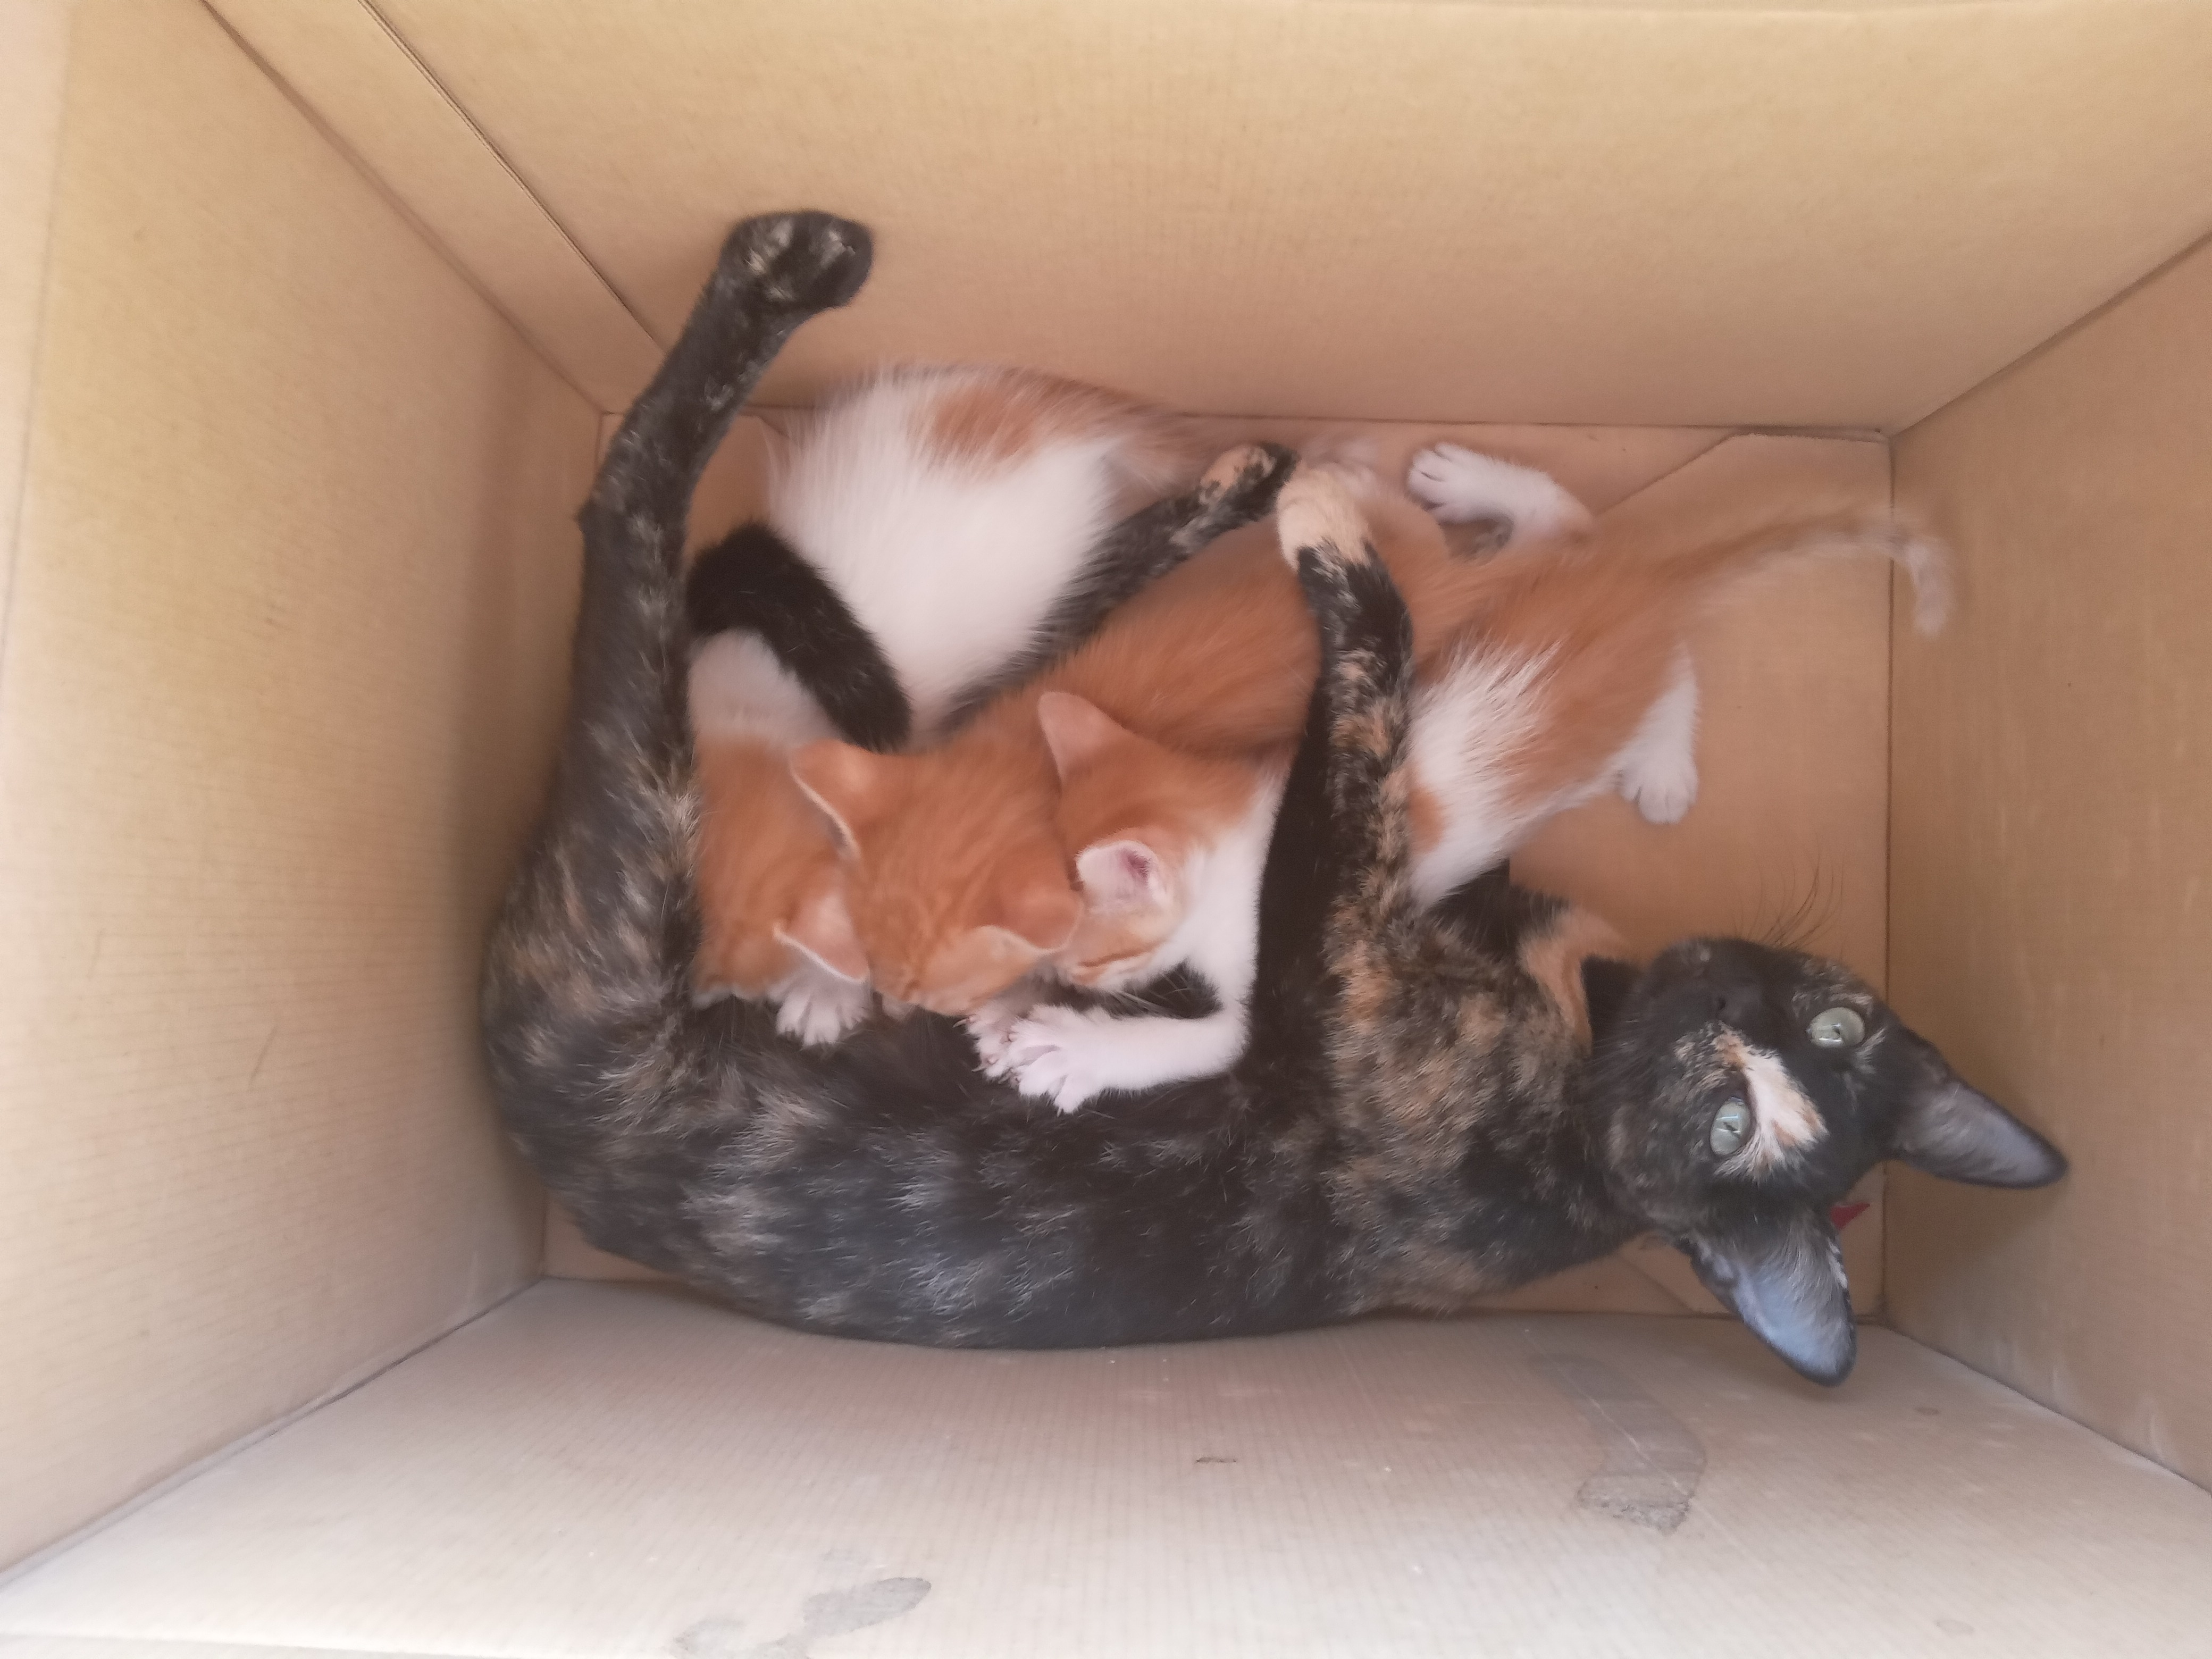
\includegraphics[width=0.9\textwidth]{figures/puppies.jpg} \\

\noindent One Monday in February, the nineteenth day of the month, I decide to get in the car very early in the morning and go make about an hour and thirty trip to buy cat food at the distributor. The puppies are growing up and will soon need to be fed with more than mother's milk. I haven't looked after puppies for a long time, so I lost track of the right weaning period. \\

\noindent When I arrive at the distributor, I discover that I cannot make the purchase order because, hours before, someone cut the wire that takes the internet to the company. \\

\noindent I keep talking to the saleswomen, hoping that the situation will somehow be resolved. With a strong tone of happiness, I tell them about the birth of the kittens and the curious fact that Joana made her nest inside the wood of an old crate-type bed that I left in the Cattery. My other kittens pierced the wood from the top, providing a perfect refuge for Joana. \\

\noindent I get home a little after lunchtime. I'm working late to make up for the time I've wasted buying the cat's food. I end the day pleased to have finally managed to finish the introduction of one of the two articles that were approved for a scientific congress. I read the introduction, and I see that it is not perfect, but finally the text is very good. Few final modifications will be made. I can finally move on to the next sections. I think that the introduction of an article is always the most difficult and time-consuming part of writing and that I will not have great difficulties to finish the work on time. I'm going to sleep satisfied with myself. \\

\noindent Tuesday morning I wake up early and go take care of my kittens. I have a habit of always counting all the kittens before leaving the Cattery, to make sure everyone is safe and protected. I count each one making sure to fill them with affection while I do the conference. Charlotte, Mimi, Nina, Saça, Braquinha, Raposinha, Mel and the babies Pingo, Lyon, Joheau, Denguinho, Bruce and Joana. Then I look into the wood of the bed and am glad to see that Joan's four children are already walking better and biting each other. \\

\noindent I realize that I will not have time for breakfast. I hurriedly take a shower, get ready and go to work. \\

\noindent After class I return home excited to continue crafting the article. When I get home I leave my bags and go into the Cattery to take care of the kittens. \\

\noindent I play a little with the older kittens and then I realize that one of Joana's puppies is not inside the bed bin. I'm looking all over the Cattery. I look for every inch of the Cattery and I can't find it. I remember that when I entered the Cattery, I noticed that the kittens were very communicative and that this happened whenever they went through an unexpected situation.  \\

\noindent I think there is no way a kitten thirty days old, who had not even weaned, could escape from the Cattery. But still I go out of the Cattery and search the grounds of my house, then I go back and search inside the Cattery again. I do this several times, repeatedly. \\

\noindent Then I remember the employees who are doing work in the condominium. I remember the various other problems I have suffered since the work began. I remembered the attacks I had suffered in the last two years. Physical and psychological torture. Everything passes in my mind like a movie and I understand what is happening. \\

\noindent I get very stressed when I realize that someone just walked into the Cattery while I was working and took one of Joan's puppies. I go to the construction workers and ask about the kitten. I ask permission and enter the condominium guardhouse to look for it. I find that the employees of the construction site are installed in the guardhouse as if they were living there. Which is absurd, considering that it is the guardhouse of the condominium. But I can't find my kitten. I see one of the employees walking away with a backpack on his back. The construction workers inform me that he is going to receive a payment. \\

\noindent I'm going to the police station to file a complaint. I try to explain everything as best as possible. \\

\noindent The next day I wake up in the morning. I realize that the employees are using, in the work of the condominium, the sand that I bought to make the wall and the fence on my land. I had already warned them that that sand is mine and that they should not use it. It seemed to me a provocation. I took pictures. I went to the police station again, as I was informed that the police delegate would be there on Wednesday morning. But I didn't get to talk to him until Thursday. \\

\noindent On Wednesday I discussed this issue with my lawyers. \\

\noindent On Thursday morning, I sent all the photos I had, a video and a narrative description made in a notary's office narrating about most of the problems I had with the condominium work. \\

\noindent I had already talked to the man responsible for the condominium work about all the problems and, after our conversations, I believed that they would be solved. I was informed that the position of the curb would be corrected. But when I left the house, I saw that the construction workers were laying cement for fixing the curb, disrespecting the width of the sidewalk near my house. I had a strong discussion with the staff. I had no doubt that this was being done to harm me. To affect my psychological state. But after the theft of my kitten, the aggression that this meant for me, taking from the mother a little animal that had not even been weaned, certainly to abandon somewhere and let him starve. After that there was no way not to stress and the discussion was right. \\

\noindent I tried to explain to them that they should use Square and measure the width of the street, and the sidewalk, always leaving the same distance. But they started being rude to me and I started arguing with the three workers. I realized they were recording the discussion with a cell phone. The construction workers at the condominium began making false insinuations. I realized they were trying to use the recording to incriminate me. \\

\noindent Suddenly the lady, who is the current companion of the Lord who sold me the land of the condominium and is causing me so much trouble, appeared, appeared out of nowhere and began to argue with me. An 80-year-old lady told me to shut up several times and started making innuendos. With allegations of things that she should not have known about, such as the fact that I have gone to the police station several times to make several complaints about different assaults that I have suffered. \\

\noindent It was an awkward moment. But the behavior of this lady made me understand what was happening. The theft of my kitten with only thirty days, as well as the use of sand that I bought for the condominium work, and the insistence on the improper placement of the curb. They were provoked actions so that I would exasperate myself so that they could create evidence against me. \\

\noindent I came out of that terrible environment and went to talk to the police delegate. Who was very kind to listen to me carefully and try to understand everything I was suffering in the last 26 months, as well as previous problems. \\

\noindent The delegate made me sign a term of cooperation and told me that this problem would be discussed judicially. \\

\noindent And my thirty-day-old kitten ... ? After 36 hours, I can't believe there's anything I can do for it. \\

\noindent I can only ask God to take care of it or its feline soul and that there be justice. \\

\noindent I hope God hears me. And let these criminals pay for their crimes. \\

\noindent At the police station I noticed a poster about the murder of a girl. In the photo a beautiful young woman smiling, above the photo a message: "there is no perfect crime". Below the photo, request for complaints to determine the crime. \\

\noindent When I saw this poster, I thought: this is just one of thousands of paintings from Brazil. \\

\noindent Friday morning, I really want to work, but I can't continue to write the article. I feel like I'm in shock. There are no ways to describe my anguish and suffering. I remember the kitten that was stolen. Beautiful, all white, but with a little beige at the top of the tail, as if such a beige strip had been created to attest to his kinship with his little brothers. I remember him joking. \\

\noindent The stolen kitten was the only one (entre os quatros) that I had ever been given a name. I gave it the name Xodó. Even though it's almost all white. I could recognize the soul that was inside it. Xodó is the name of a cat I had in my childhood. I was totally in love with this cat. The Xodó of my childhood was all black. Absurdly beautiful. I had another Xodo, completely black and also absurdly beautiful, with eyes of a dense green. Charlotte's brother. \\

\noindent Xodó, brother of Charlotte and Tigre, disappeared from my apartment and was, in this way, responsible for the fact that I adopted so many kittens. But that's another story that will be told in another chapter ... \\

\chapter{Why COVID was created ?}

... latter ....

\chapter{In the middle of the stones flowers are born}

\noindent For me, one of the most unforeseen outcomes of Game Of Thrones was that I simply became addicted to chatting in game chats. \\

 \noindent The first few times, it was out of sheer need for survival in the game. It was really some kind of overcoming. \\

\noindent But I soon discovered that in the middle of all that confusion of mixed phrases and nonsense, it was possible to filter dialogues and that there was a story there, of which I could be part. \\

\noindent And this addiction became much worse after I met KanT, a colonel in the Russian army, extremely intelligent and intellectual, who loved flipping through war books. At the time, new leader of the KgB.  \\

\noindent Oh... my eyes filled with fascination at the sight of the sudden attacks of the KgB, destroying everything on the map. \\

\noindent KanT became my partner, KgB my most important ally. Then... I created a new character and infiltrated the KGB alliance, after I became k116's Queen. \\ 

\noindent With KanT were always long conversations, and between them, I could not wait for the next meeting ... \\

\noindent One day KanT explained to me in great detail the difference between instinct and intuition. Then he told me that few people had these two well-developed natural defense tools. But that I have both. \\

\noindent For a long time, after 2022, I had by intuition or instinct, a strong thought telling me that I should speak openly about what was happening to me. \\

\noindent And, at some point, these feelings were so strong, I gave in. I created a video talking about the fact that I was terrorized, kidnapped and held in private prison in a hospital for 23 days. I posted the video on youtube. \\

\noindent After that, the battle I was being forced to fight became more pronounced. My life has become a real hell. \\

\noindent But today I clearly see that at that time someone needed to talk about it. \\

\noindent It would be a really good thing if all the people who felt wronged had something to say about and, in one way or another, spread their words to the world. \\

\noindent The problem is that people are being agressed, tortured, when talking. \\

\noindent The other day we were talking about religion and I asked KanT: do you believe in hell ? He replied: there is so much evil in the world that there must be a hell ... it is not possible that there are such cruel people and that there is no punishment for such cruelty either in life or after life. \\

\noindent I remember KanT writing this sentence and then I think about how much the story of Christ repeats itself. I do not understand why Christ said: God, forgive them ... But Christ was a holy man ... and surely I would never be able to comprehend all his wisdom. \\

\noindent Today, when I see the phrase:

\noindent \begin{center} \emph{together we are strong !} \end{center}

\noindent I feel bad and force myself to ask the question:

\noindent \begin{center} \emph{together against whom ?} \end{center}

\noindent The philosophy of "together we are strong" amazes me more than it convinces me. \\

\noindent It's not a question of togetherness. But it's a matter of strength.

\noindent \begin{center} \emph{It's not to do together. It's for everyone to do their part.} \end{center} 

\noindent And, I am glad to see that, although belatedly, the effect of neo-politics has been exactly that of provoking an anti-neo-politics. \\

\noindent This became clear to me a few minutes ago when I went to look up the meaning of the word \emph{Decoloniality}. \\

\noindent Imperialism mixed with patriarchy, and the exploitation of everything, even living beings and life itself, as a source of capital can have no result but revolt. \\

\noindent But this time, the revolt came as an intellectual response, from intellectuals. \\

\noindent Questions and counterproposals of intellectuals concerned with the planet and society, for the planet and society themselves . \\

\noindent \begin{center} \emph{Maybe it will take time to happen, but I see drawing itself the hope of a different future} \end{center}

\chapter{Evolution based on experience}

At some point in human history, Charles Darwin wrote: 

\chapter{Is Brazil experiencing a new period of dictatorship ?}

\noindent I posted this question on duckduckgo.com and, digging around, I found a report from the Latin America Bureau (LAB) posted on May 1, 2014 entitled "Brazil: the spirit of dictatorship is alive and well". \\

\noindent The newspaper recounts a dark moment in Brazil's history when a planned coup was beginning to be put into effect. Almost as if it presented an enigmatic prediction about the terrible times to come. \\

\noindent Such a moment was succeeded by a chain of events, including the spread of a terrible supposed pandemic which was accompanied by absurd technological development that managed to make Moore's law obsolete. \\

\noindent Reading this article has caused me enormous grief. And while I started writing I had to deal with a strange and uncomfortable sensation of sharp pain and tingling in the head, near the nape of the neck. This feeling is becoming stronger as I insist on reporting my reflections. But I don't give up writing. \\

\noindent Is Brazil experiencing a new period of dictatorship ? I repeat the question to myself. \\

\noindent I think a little about my limited ability to answer such a question. First there is the need to understand the real meaning of the word dictatorship. \\

\noindent I dig a little deeper and find another article on this topic. It is a recent report, posted on May 3, 2024 on the France24 website. The report is titled "Brazil still struggles with the dark period of military dictatorship, 60 years later". \\

\noindent The report is presented in a video. Some people of somewhat advanced age narrate about a dark period in which they were arrested by the government, locked in buildings and tortured. \\

\noindent According to the free encyclopedia Wikipedia, the regime established in Brazil on April 1, 1964 and lasting until March 15, 1985, later recognized as the Brazilian military dictatorship, was marked by the inhibition of political discourse through torture and murder.

\noindent \begin{center} \emph{Absurd aggressions, but visible.} \end{center}

\noindent Is Brazil experiencing a new period of dictatorship ? I repeat the question to myself. \\
 
\noindent Yes, people are being subjected to some kind of torture and yes people are being silenced.

\noindent \begin{center} \emph{Absurd aggressions, and invisible.} \end{center}

\noindent When I can put myself short out of this madness, I think of the teachings of mester Sun Tzu, in his book "The Art of War". Then it becomes clear to me that there is something behind all this.

\noindent \begin{center} \emph{What is behind all this ?} \end{center}

\noindent It seems that such nonsense was now justified by the pursuit of technological progress. \\

\noindent Is Brazil experiencing a new period of dictatorship ? I repeat the question to myself ...

\noindent \begin{center} \emph{Is the world experiencing a new period of dictatorship ?} \end{center}

\noindent Perhaps, this question is not the most relevant question. \\

\noindent I believe that at this point, world governments are already aware of the use of people as guinea pigs for data collection that will be used to feed the training and testing of new and diverse neural networks. Whose learning becomes deeper and deeper. The objects of the studies range from thinking and the origin of ideas to the behavior of proteins and microbiota and the impact of this on various forms of life, including human lives. \\

\noindent Perhaps, the most relevant question is:

\noindent \begin{center} \emph{How many lives will still be destroyed to meet all the nonsense of society ?} \end{center}

\noindent And the Brazilian government distracted by an incessant fight against fake news.

\noindent \begin{center} \emph{"Here is what I had to say about the different advantages you must try to obtain when, in command of the army, you will have to measure yourself against enemies perhaps as prudent and valiant as yourself. They cannot be beaten unless you use the little stratagems I have just indicated."
[by Sun Tzu - Art Of War]} \end{center}

\chapter{Why COVID was created ?}

No caso do argumento que segue, tenho intenção de provar, usando lógica, que: \\

\noindent \begin{center} \emph{é possível (provável) que o COVID tenha sido criado intencionalmente para alavancar o desenvolvimento de novas tecnologias.} \end{center}

A tese que segue nas próximas linhas foi desenhada com base nos seguintes argumentos lógicos: \\

Houve um avanço absurdo relacionado ao desenvolvimento de novas tecnologias; \\

O desenvolvimento de algumas das novas tecnologias só poderia acontecer com base em uma absurda quantidade de dados humanos; \\

Os nanomaterias tem tamanhos na escala das células e podem também ser usados para "coletar" pensamentos (em 2019, havia tecnologia embrionária para tanto); \\

Dados humanos a nível celular podem ser adquiridos com nanotecnologia (em especial nanorobótica, mas não somente); \\

Os nanomaterias são geramente inseridos no corpo através de injeção; \\

O COVID se difundiu através do mundo sem nenhum controle, apesar do sar cov não ser um vírus desconhecido; \\

Meios de comunicação geraram pânico em torno do assunto inclusive informando erroneamente à operários de empresas que estes eram obrigados a se vacinar; \\

Uma grande percetangem das pessoas em nosso planeta receberam injeção de forma voluntária ou obrigatória por causa do pânico gerado em torno do COVID; \\

No Brasil, as injeções (vacinas) começaram a ser administradas em grupos e não como deveria ocorrer em uma pandemia; \\

A vacina não parece ter reduzido as taxas de transmissão e morte causados pelo vírus; \\

As pessoas tiveram sintomas que foram atribuídos ao COVID; \\

As sintomas "do COVID" se assemelham aos sintomas indentificados no uso de nanomateriais. \\


\noindent \begin{center} \emph{Portanto, se isso é fato, COVID foi a maior mentira e, possivelmente, um dos maiores genocídeos de nossa era.} \end{center}

\noindent \begin{center} \emph{Ontem eu descansei e antes de dormir eu estava bem e descansada. Decidi que hoje eu tiraria o dia para arrumar a casa ... mas como transformaram meus domingos e a minha vida em um inferno ... e transformaram algumas de minhas noites em uma verdadeira tortura ... estou aqui escrevendo ... e por todas as outras pessoas que sofreram e estão sofrendo uma parte do que eu tenho tido que suportar, espero poder continuar a escrever ...} \end{center}

Este capítulo será um capítulo longo. \\
Devido à complexidade e relavância do tema, vou apresentar um forte embasamento bibliográfico. \\
A discussão será desenvolvida durante vários dias (ou semanas). \\
Pois para tanto será necessário uma longa pesquisa. \\

Mas segue relação dos temas que estou desenhando para este capítulo. \\

se existe alguma duvida sobre o COVID ter sido criado; \\
convergências e divergências entre as ciências direito e matemática; \\
a relação entre os sintomas do COVID e os sintomas que são causados pelo uso de nanomateriais; \\
meios de imformação e a alienação humana; \\
A relação sobre o COVID e a política do horror. \\

A ridiculação do pensamento crítico e a resignificação do termo negacionismo. \\

Por que accredito que empresários e cientístas criaram e espalham o COVID (ou o medo do COVID) ? \\

- levantamento de dados; \\
- desenvolvimento de tecnologia, em especial nas áreas de robótica e biociência; \\
- desenvolvimento de inteligências (cérebros) artificias; \\
- computação de altíssimo desempenho usando cérebros humanos; \\
- controle sobre a informação e as pessoas; \\
- e é claro: dinheiro e poder.

\end{document}

